
% Baseado em:
% http://theoval.cmp.uea.ac.uk/~nlct/latex/thesis/node1.html

\documentclass[a4paper]{report}

% para gerar indices no pdf
\usepackage[bookmarks]{hyperref}    

\usepackage[applemac]{inputenc}
\usepackage[portuguese]{babel}
\usepackage[T1]{fontenc}


% definir margens de 2 cm
\RequirePackage[a4paper,margin=2cm]{geometry}
\usepackage{graphicx} 

\usepackage[tikz]{bclogo}
\usepackage{verbatim}

\usepackage{lastpage}
\usepackage{fancyhdr}
%\setlength{\headheight}{15.2pt}
\pagestyle{fancyplain} { % define first page header and footer
%\fancyhead[L]{Course Report}
%\fancyhead[C]{Manual de Utiliza��o OpenK POS}
%\fancyhead[R]{\thepage of \pageref{LastPage}}
\fancyfoot[L]{Alexandre Bragan�a}
\fancyfoot[C]{(c) KTC Lda / www.openk.pt}
\fancyfoot[R]{\thepage}
}


\begin{document}

\title{Manual de Utiliza��o do OpenK POS}
%\author{Alexandre Bragan�a}
\author{Alexandre Bragan�a\\
  KTC Lda,\\
  Rua EN 327, 1315
  4520-706 Souto, Santa Maria da Feira,\\
  Portugal,\\
  \texttt{alexandre.ktc@gmail.com},\\
  \texttt{www.openk.pt}}
\date{Dezembro 2013}

\maketitle

\pagenumbering{roman}
\tableofcontents
\listoffigures
%\listoftables

%\chapter*{Agradecimentos}

%\begin{abstract}
%\end{abstract}

\newpage

\pagenumbering{arabic}

\chapter{Apresenta��o}
\label{ch:apresentacao}

Neste manual encontrar� informa��o sobre como administrar e operar o OpenK POS
\cite{openk}. 
O OpenK POS � um software de fatura��o e posto de venda que se baseia no
Openbravo \cite{openbravo}, um dos softwares de gest�o \emph{open source}
(software aberto e livre) mais usado em todo o mundo.

O OpenK POS est� devidamente certificado pela DGCI/AT (Dire��o Geral de
Contribui��es/Autoridade Tribut�ria) tendo a licen�a de certifica��o n�1345. O
OpenK � uma adapta��o para o mercado portugu�s do Openbravo, o software de
gest�o aberto e baseado em tecnologia internet l�der mundial com mais de 2000000
de utilizadores. Existem centenas de grandes empresas em diversos pa�ses a
utilizarem com grande sucesso esta solu��o. No retalho destaca-se como
refer�ncia o caso da BUT, a empresa francesa l�der da distribui��o de m�veis em
Fran�a, com uma solu��o de mais de 1000 postos de venda Openbravo POS. O OpenK
POS � a vers�o portuguesa do Openbravo POS certificada pela DGCI/AT e adaptada
para o mercado nacional.

\begin{figure}[h!]
  \centering
      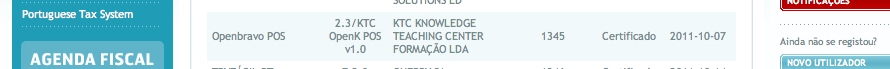
\includegraphics[width=0.8\textwidth]{./imgs_org/certifica_at.png}
  \caption{Apresenta��o do certificado do OpenK POS no site da AT}
\end{figure}

\begin{figure}[h!]
  \centering
      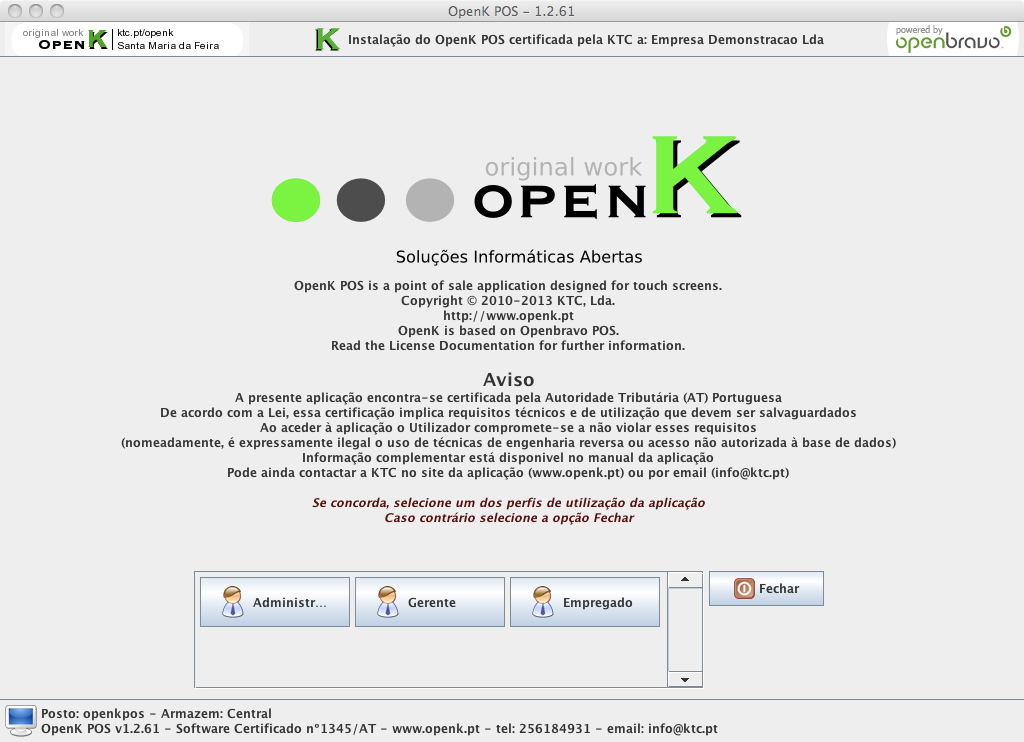
\includegraphics[width=0.8\textwidth]{./imgs_org/init_app.png}
  \caption{Janela de abertura da aplica��o}
\end{figure}

\section{Caracter�sticas}
Salientamos as seguintes caracter�sticas e funcionalidades do OpenK POS:\\
\\Garantia
\begin{itemize}
	\item Software Certificado pela AT com emiss�o de ficheiros SAF-T PT
	\item A garantia de utilizar um software l�der mundial
\end{itemize}
Gest�o de Dados
\begin{itemize}
	\item N�mero ilimitado de clientes e produtos
	\item Possibilidade de defini��o de impostos (ex: IVA) diferentes por cliente
	\item Possibilidade de definir produtos compostos
	\item Possibilidade de definir produtos com atributos (Ex: cor e tamanho)
	\item Multi-utilizador
	\item Possibilidade de definir cart�es para colaboradores e clientes 
\end{itemize}
Vendas, Devolu��es e Gest�o de Caixa
\begin{itemize}
	\item Emiss�o de tal�es de caixa e faturas configur�vel
	\item M�ltiplos recibos em um ou mais terminais
	\item Divis�o de recibos
	\item Gest�o de conta correntes de clientes
	\item Gest�o vers�til de devolu��es
	\item M�ltiplos modos de pagamento
\end{itemize}
Gest�o de Stocks e Armaz�ns
\begin{itemize}
	\item Gest�o de stock de produtos (registo de entradas, sa�das e movimenta��es)
	\item Stock de produtos automaticamente actualizado
	\item Suporte para m�ltiplos armaz�ns
	\item Gest�o de stocks com base nos atributos dos produtos	 
\end{itemize}
M�dulo de Restaurantes e Caf�s
\begin{itemize}
	\item \emph{Layout} interativo de mesas
	\item Gest�o de reservas de mesas
	\item Possibilidade de utiliza��o de m�dulo adicional para Smarthone/PDA/Tablet
\end{itemize}
Relat�rios e Gr�ficos
\begin{itemize}
	\item Relat�rios e graficos configur�veis
	\item Vendas por utilizador
	\item Vendas por produto
	\item Stocks
	\item Dividas de clientes
	\item Imposto liquidado
	\item e muito mais.
\end{itemize}
Especifica��es T�cnicas
\begin{itemize}
	\item Multi-posto
	\item Multi-plataforma: Windows, Linux e Mac OSX
	\item Funcionamento com ecr�s t�cteis
	\item Funcionamento com leitores de c�digos de barras
	\item Funcionamento com balan�as
	\item Funcionamento com impressoras de POS
\end{itemize}

\section{Funcionamento em Rede}
A aplica��o permite um ou mais postos. Cada posto tem o seu nome que � derivado
do nome do computador. Os postos trabalham em rede, partilhando os mesmos
dados.

Um posto acede aos recibos dos outros postos quando arranca. Em cada momento
apenas um posto deve trabalhar com um recibo. A vers�o que fica de um recibo � a
do �ltimo posto que o alterou.

O nome do posto (atribu�do no ficheiro de propriedades) � usado para identificar
o caixa, e � usado nos fechos de caixa. Este aparece na faixa do final do ecr�
(assim como o armaz�m activo).

\section{Estrutura do manual} 

Este manual esta estruturado de forma a facilitar a sua consulta pelo
utilizador.

No cap�tulo 2 encontra informa��o sobre a instala��o e configura��o da
aplica��o.

No cap�tulo 3 encontra a descri��od e como funcionam na generalidade os ecr�s da
aplica��o.

No cap�tulo 4 encontram-se descritas as funcionalidades que permitem administrar
a aplica��o.

No cap�tulo 5 encontram-se descritas as funcionalidades da aplica��o para os
operadores da aplica��o.

O cap�tulo final informa sobre a licen�a da aplica��o.


%\begin{center} 
%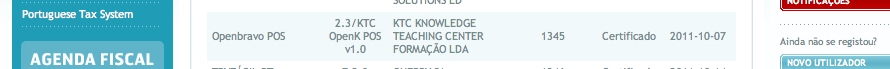
\includegraphics[width=140mm]{./imgs_org/certifica_at.png}
%\end{center}

% Isto é um exemplo de citação \cite{goossens97}.

%@startuml intro.png
%
%(First usecase)
%(Another usecase) as (UC2)  
%usecase UC3
%usecase (Last\nusecase) as UC4
%
%@enduml

%@startuml seq1.png
% participant User
% User -> A: DoWork 
% activate A #FFBBBB
% A -> A: Internal call 
% activate A #DarkSalmon
% A -> B: << createRequest >> 
% activate B
% B --> A: RequestCreated 
% deactivate B 
% deactivate A 
%A -> User: Done 
% deactivate A
%@enduml

%\begin{center}
%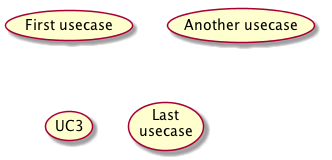
\includegraphics[width=80mm]{./imgs/intro.png}
%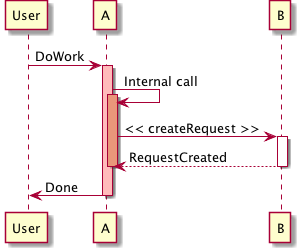
\includegraphics[width=80mm]{./imgs/seq1.png}
%\end{center}

\chapter{Instala��o e Configura��o}
\label{ch:instalacao}

\indent A instala��o e configura��o deve ser sempre efectuada por t�cnicos da
KTC.
\newline
\newline
\noindent A instala��o contempla:
\begin{itemize}
	\item hardware (perif�rios)
	\item java
	\item servidor de base de dados
\end{itemize}
\noindent A configura��o contempla:
\begin{itemize}
	\item configura��o dos diversos postos
	\item dados de empresa
	\item armaz�ns
	\item \emph{layout} dos documentos
	\item utilizadores e permiss�es
\end{itemize}


\chapter{Interface da Aplica��o}
\label{ch:interface}

Nesta sec��o do manual apresentam-se e explicam-se as principais caracter�sticas
da interface da aplica��o, isto �, da forma como a aplica��o interage com o
utilizador.\newline
\indent O OpenK POS � uma aplica��o vocacionada para a intera��o baseada em
ecr�s t�cteis. Assim, a disposi��o dos elementos no ecr� e a sua dimens�o est�o
adaptados a esta situa��o.\newline

\begin{figure}[h!]
  \centering
      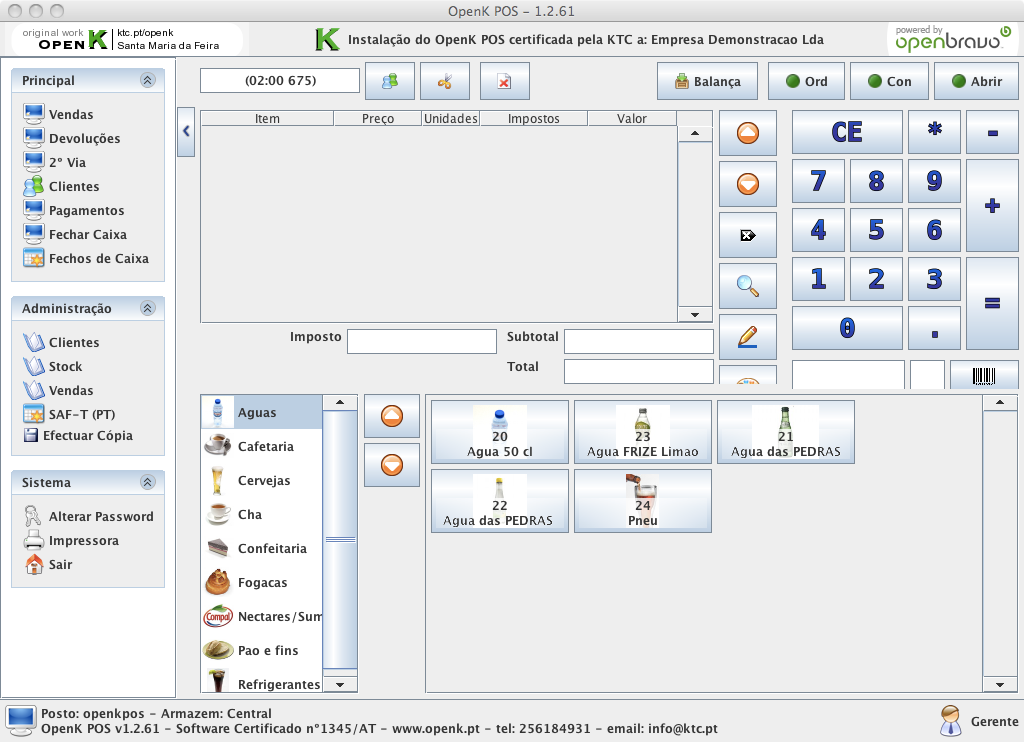
\includegraphics[width=0.8\textwidth]{./imgs_org/main_win.png}
  \caption{Interface da aplica��o}
  \label{fig:main_app}
\end{figure}

\noindent A Figura ~\ref{fig:main_app} ilustra o aspecto usual da
interface da aplica��o. O ecr� est� dividido em tr�s partes: uma coluna lateral esquerda na qual aparecem as
op��es disponibilizadas para o perfil do utilizador; uma �rea maior, � direita,
na qual se apresenta o conte�do relativo � op��o actual (no caso ilustrado na
Figura ~\ref{fig:main_app} a op��o activa � da \emph{Vendas}) e uma pequena �rea
na parte inferior do ecr� inde aparece a informa��o sobre a aplica��o, a identifica��o do
utilizador actyal, o armaz�m actual e o nome do posto.

\section{Barra de Navega��o}
Nas janelas que permitem trabalhar com v�rios registos � comum a utiliza��o de
uma barra de bot�es com a ilustrada na Figura ~\ref{fig:nav_bar}.\newline

\begin{figure}[h!]
  \centering
      
\includegraphics[width=0.8\textwidth]{./imgs_org/nav_bar.png}
  \caption{Barra de bot�es de navega��o}
  \label{fig:nav_bar}
\end{figure}
\noindent As funcionalidades da barra (da esquerda para a direita) s�o as
seguintes:
\begin{itemize}
	\item N�mero do registo actual / N�mero total de registos
	\item Movimentar para o primeiro registo
	\item Movimentar para o registo anterior
	\item Carregar o registo original (pedendo os dados alterados)
	\item Movimentar para o pr�ximo registo
	\item Movimentar para o �ltimo registo
	\item Carregar todos os registos
	\item Pesquisar registo
	\item Ordenar os registos
	\item Criar novo registo
	\item Remover o registo actual
	\item Guardar o registo actual
\end{itemize}

\section{Relat�rios}
A aplica��o contempla os mais diversos relat�rios para a extra��o de
informa��o. � poss�vel imprimir ou guardar os relat�rios em diversos
formatos.\newline



\chapter{Administra��o}
\label{ch:administracao}

\section{Utilizadores}
O OpenK POS v�m configurado com 3 tipos de utilizadores: o
Administrador (reservado � assist�ncia por parte da KTC); o Gerente (o
utilizador com mais permiss�es) e o empregado (um utilizador com menos
permiss�es, basicamente s� podendo efectuar opera��es relacionadas com
vendas).\newline
\indent A Figura ~\ref{fig:opcoes_gerente} e a Figura
~\ref{fig:opcoes_empregado} ilustram, respectivamente, as op��es dispon�veis para o utilizador Gerente e para o utilizador Empregado.\newline

\begin{figure}[ht]
\begin{minipage}[b]{0.45\linewidth}
	  \centering
	      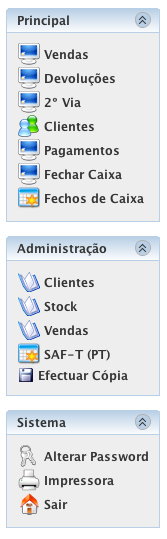
\includegraphics[width=0.4\textwidth]{./imgs_org/opcoes_gerente.png}
	  \caption{Op��es do gerente}
	  \label{fig:opcoes_gerente}
\end{minipage}
\hspace{0.5cm}
\begin{minipage}[b]{0.45\linewidth}
	  \centering
	      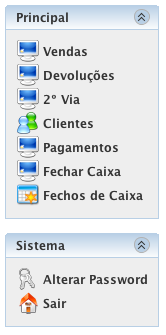
\includegraphics[width=0.4\textwidth]{./imgs_org/opcoes_empregado.png}
	  \caption{Op��es do empregado}
	  \label{fig:opcoes_empregado}
\end{minipage}
\end{figure}

\begin{bclogo}[couleur=blue!30, arrondi=0.1, logo=\bclampe, ombre=true]{�
poss�vel criar novos utilizadores e/ou alterar os existentes} Como esta funcionalidade tem implica��es ao n�vel da
seguran�a da aplica��o deve ser efetuada por t�cnicos da KTC a pedido do
cliente.
\end{bclogo}\newline

\noindent As configura��es poss�veis sobre os utilizadores incluem as suas
permiss�es, a associa��o de um cart�o de utilizador ou a associa��o de uma fotografia. Se o
utilizador tiver um cart�o associado � poss�vel efetuar o login por leitura do
c�digo de barras do cart�o do utilizador.

\section{Armaz�ns}
Apesar de ser poss�vel definir v�rios armaz�ns e um produto existir em v�rios
armaz�ns cada POS apenas trabalha com stock de um �nico armaz�m. Essa defini��o
� efetuada aquando da instala��o do OpenK POS.\newline

\begin{bclogo}[couleur=blue!30, arrondi=0.1, logo=\bclampe, ombre=true]{�
poss�vel definir mais do que um armaz�m} Como esta funcionalidade tem
implica��es ao n�vel da seguran�a da aplica��o deve ser efetuada por t�cnicos da KTC a pedido do
cliente.
\end{bclogo}

\section{Impostos}
O OpenK POS suporta um elevado n�vel de flexibilidade no que se refere a
impostos. � poss�vel definir impostos n�o s� por produto mas tamb�m por cliente.
Para al�m disso � ainda poss�vel definir mais do que uma taxa de imposto para o
mesmo produto.\newline
\indent As situa��es descritas anteriormente, embora poss�veis, s�o pouco
comuns, pelo que o OpenK vem configurado com as 3 taxas de IVA normais para
Portugal continental: Taxa Normal, Taxa Interm�dia e Taxa Reduzida.\newline
\indent As opera��es relativas � defini��o de impostos est�o acess�veis atrav�s
da op��o de administra��o \emph{Stocks}.\newline
\indent De seguida descrevem-se os passos gerais que constituem a defini��o de
impostos.

\begin{figure}[h!]
  \centering
      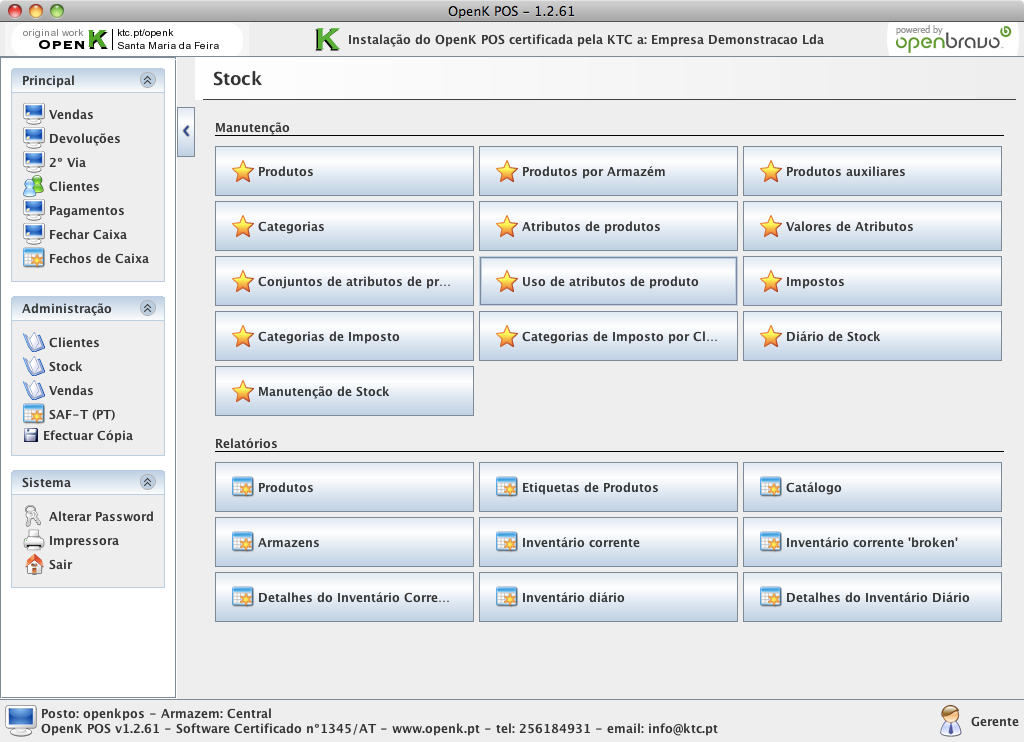
\includegraphics[width=0.8\textwidth]{./imgs_org/main_stocks.png}
  \caption{Op��es de administra��o relacionadas com stocks e produtos}
\end{figure}

\subsection{Categorias de impostos por cliente}
Este passo � opcional. Permite definir categorias de impostos que podem ser
associadas a clientes. Desta forma ser� poss�vel ter impostos (taxas) diferentes
por tipo de cliente. Permite, por exemplo, aplicar taxas diferentes para
clientes das regi�es aut�nomas ou dos pa�ses membros da Uni�o Europeia. Como se
pode observar pela Figura ~\ref{fig:cat_imp_cli} a sua defini��o consiste
apenas na atribui��o de uma designa��o para uma categoria.\newline

\begin{figure}[h!]
  \centering
      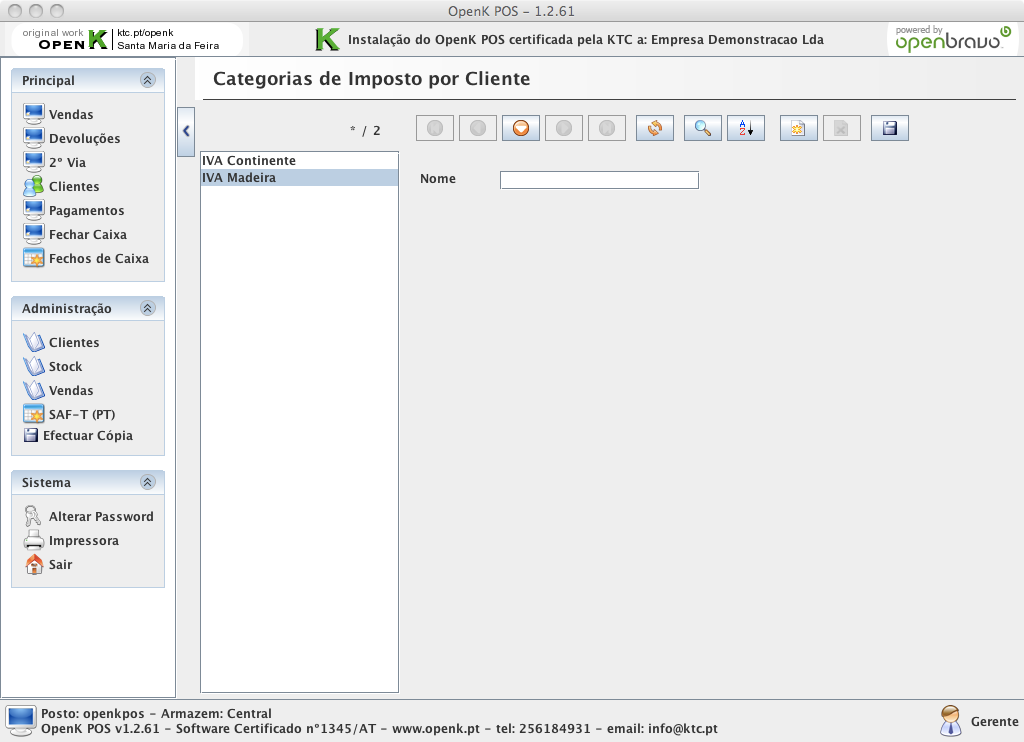
\includegraphics[width=0.8\textwidth]{./imgs_org/cat_imp_cli.png}
  \caption{Janela de defini��o de categorias de imposto por cliente}
  \label{fig:cat_imp_cli}
\end{figure}

\subsection{Categorias de impostos}
Este passo � obrigat�rio. � necess�rio definir categorias de impostos uma vez
que cada produto deve pertencer a uma categoria de imposto. Podemos, por
exemplo, ter um produto na categoria de ``Iva Taxa Normal''.\newline
\indent O OpenK POS vem configurado com 3 categorias de imposto, relativas �s 3
taxas de IVA portuguesas: Taxa Reduzida, Taxa Interm�dia e Taxa Normal.

\begin{figure}[h!]
  \centering
      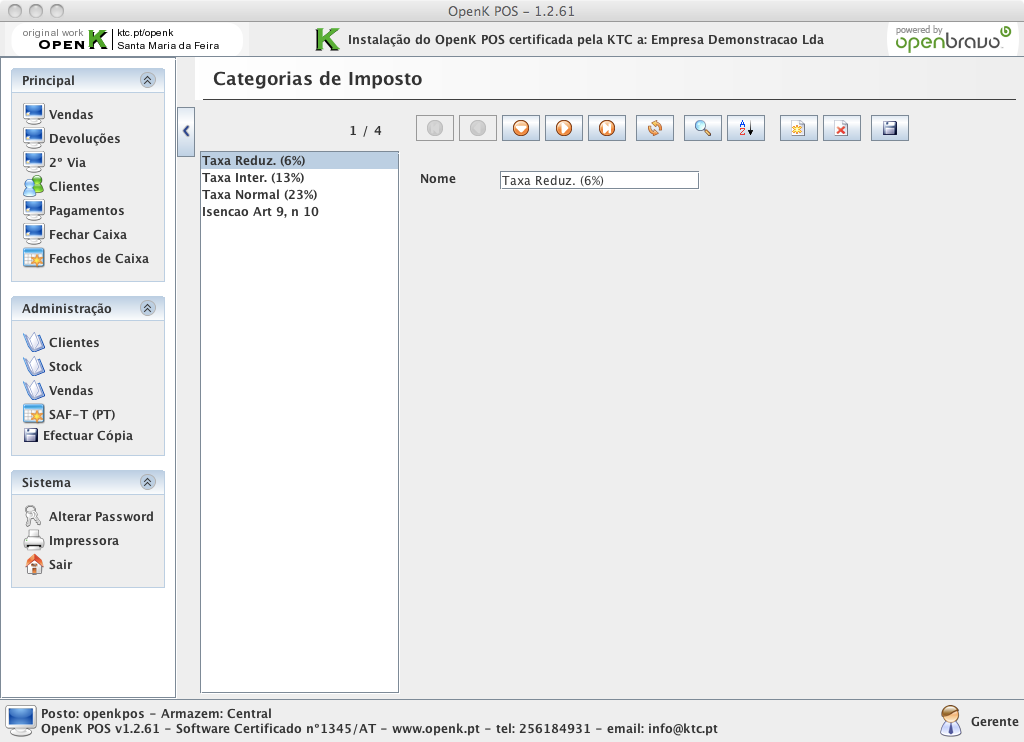
\includegraphics[width=0.8\textwidth]{./imgs_org/cat_imp.png}
  \caption{Janela de defini��o de categorias de impostos}
  \label{fig:cat_imp}
\end{figure}

\subsection{Impostos}
Este passo � obrigat�rio. � a este n�vel que se definem as taxas a aplicar. A
Figura ~\ref{fig:impostos} ilustra a defini��o de impostos.\newline
\indent A aplica��o permite que um imposto seja desdobrado em v�rias taxas. Esta
situa��o � usada em casos em que seja necess�rio cobrar mais do que um imposto
num produto que se vende. � apenas neste caso que se usam os campos ``Imposto
Pai'' e ``Ordem''. N�o � uma situa��o corrente em Portugal.\newline
\indent Cada imposto tem de estar associado a uma categoria de imposto. Isto
porque, como veremos mais � frente, cada produto est� associado tamb�m a uma
categoria de imposto. � desta forma que o programa determina qual a taxa
(imposto) a aplicar a um produto.\newline
\indent � poss�vel ainda definir para cada imposto a ``categoria de imposto de
cliente''. Esta defini��o � opcional, tal como j� foi referido anteriormente. Se
for definido este campo ent�o a aplica��o vai aplicar esta taxa quando um
produto da mesma categoria de imposto for vendido a um cliente dessa categoria
de imposto de cliente. Tal como foi referido anteriormente permite ter produtos
com taxas diferentes quando vendidos a clientes diferentes. A aplica��o de
inicio n�o est� configurada para trabalhar dessa forma (embora seja
poss�vel).\newline
\indent Por exemplo, podemos ter a categoria de imposto ``IVA Taxa Normal''.
Nesta categoria podemos definir mais do que um ``Imposto''. Por exemplo, o
imposto ``IVA Taxa Normal Continente (23\%)'', ``IVA Taxa Normal Madeira
(15\%)'' e ``IVA Membro UE (0\%)''. A cada imposto podemos associar uma
Categoria de imposto de cliente. Isto permite que a Taxa actual de IVA a aplicar
na venda de um produto possa depender do cliente. Conv�m ter sempre um imposto
\emph{default} para o qual n�o existe categoria de imposto de cliente para ser
usado por omiss�o nas situa��es mais comuns (isto �, para os clientes para os
quais n�o especificamos qual era a categoria de imposto de cliente).\newline

\begin{bclogo}[couleur=blue!30, arrondi=0.1, logo=\bclampe, ombre=true]{Nota
importante sobre o nome do imposto} Ao definirmos os impostos o campo ``nome''
deve conter a designa��o da taxa (por exemplo ``IVA Normal'') ou, nos casos de isen��o, a justifica��o da isen��o (por exemplo, ``Isen��o art9,
n10''). Essa informa��o vai aparecer nos documentos de venda.
\end{bclogo}

\begin{figure}[h!]
  \centering
      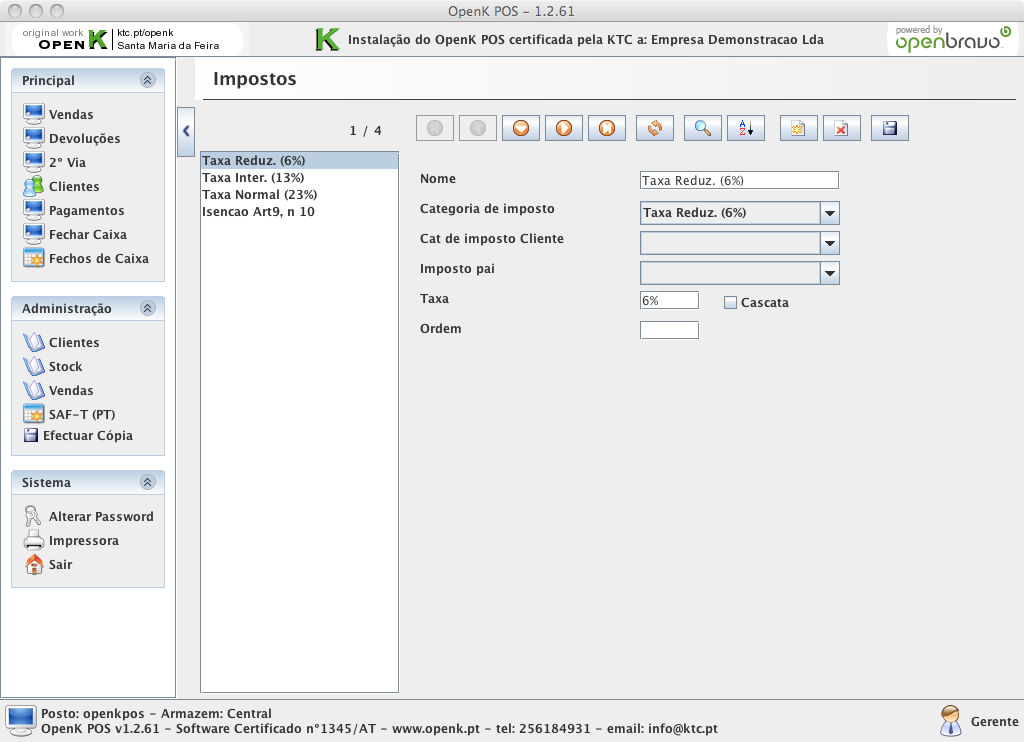
\includegraphics[width=0.8\textwidth]{./imgs_org/impostos.png}
  \caption{Janela de defini��o de impostos}
  \label{fig:impostos}
\end{figure}

\section{Produtos}

\subsection{Categorias}
� poss�vel dividir os produtos pode categorias ou classes, tal como se pode
observar na Figura ~\ref{fig:categorias}. As categorias podem ser subdivididas
em mais categorias at� ao limite desejado.\newline
\indent Para especificarmos uma categoria devemos indicar o seu nome e, caso
pretendamos que seja uma subcategoria de outra j� existente, selecionar o nome
da categoria pai no campo ``Categoria''. Pode-se ainda selecionar uma imagem
para a categoria. Esta imagem ser� apresentada depois na janela de vendas para
mais facilmente se identificar a categoria. Os bot�es adicionar e remover do
cat�logo permitem especificar se a categoria vai aparecer na janela de vendas ou
n�o e, por conseguinte, os produtos que pertenceram a essa categoria.\newline

\begin{figure}[h!]
  \centering
      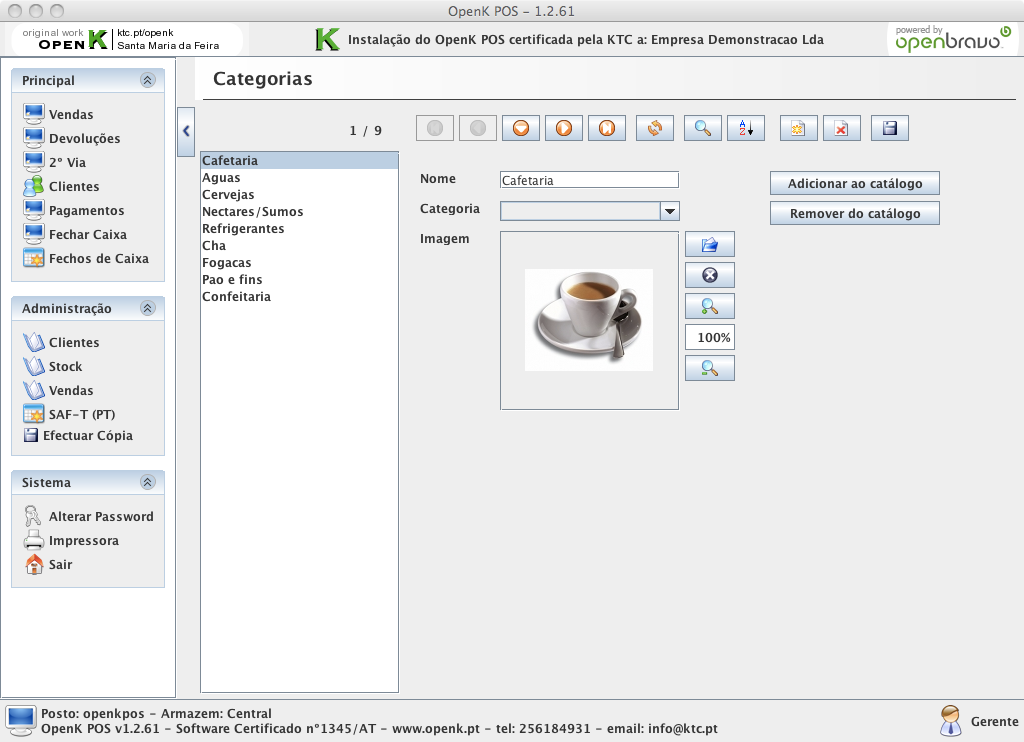
\includegraphics[width=0.8\textwidth]{./imgs_org/categorias.png}
  \caption{Janela de defini��o de Categorias de Produtos}
  \label{fig:categorias}
\end{figure}

\subsection{Atributos de Produtos}
Consiste na configura��o de atributos de produtos, como por exemplo a cor e o
tamanho. Estes dados podem depois ser usados na gest�o de stocks.\newline

\begin{itemize}
  \item (Atributos de produtos) Definir o nome dos atributos de produtos
  \item (Valores de atributos) Definir os valores poss�veis para atributos de
  produtos (se n�o se definir nenhum valor a aplica��o pede ao utilizador para
  introduzir um valor quando se usam os atributos)
  \item (Conjunto de atributos de produto) Definir o nome dos conjuntos de
  atributos de produtos
  \item (Uso de atributos de produto) Definir quais os atributos de produtos que
  faem parte dos conjuntos de atributos de produtos
\end{itemize}

\subsection{Produtos}
A defini��o de produtos � efetuada na janela ilustrada na Figura
~\ref{fig:produtos}.\newline

\begin{figure}[h!]
  \centering
      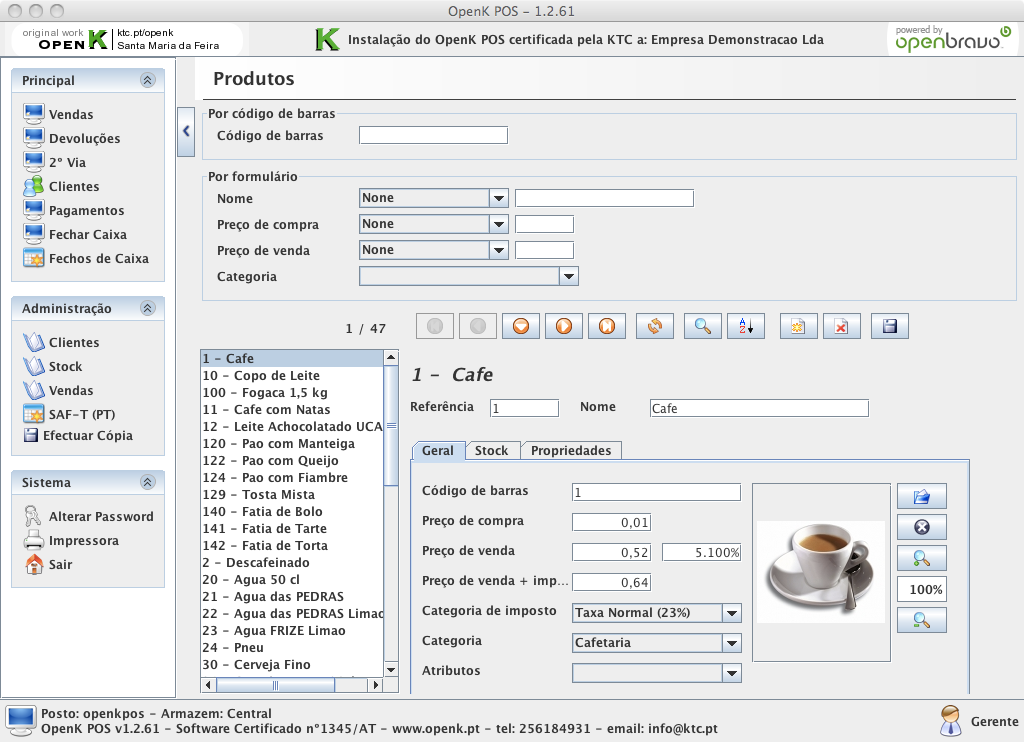
\includegraphics[width=0.8\textwidth]{./imgs_org/produtos.png}
  \caption{Janela de defini��o de Produtos}
  \label{fig:produtos}
\end{figure}

\begin{itemize}
	\item Refer�ncia = Campo usado em pesquisas
	\item Nome = Nome do Produto
	\item Geral:
	\begin{itemize}
	  \item C�digo de barras = o c�digo de barras do produto
	  \item Pre�o de compra = o pre�o de compra do produto
	  \item Pre�o de venda = o pre�o de venda do produto (sem impostos)
	  \item Margem = a margem em percentagem
	  \item Pre�o de venda + imposto = pre�o de venda ao p�blico (pre�o de venda +
	  imposto)
	  \item Categoria de imposto = a categoria de imposto a aplicar a este produto
	  \item Categoria = a categoria do produto
	  \item Atributos = o conjunto de atributos de produto a usar no produto.
	  Opcional.
	\end{itemize}
	\item Stock (ver Figura ~\ref{fig:produto_stock}):
	\begin{itemize}
	  \item Custo de stock por ano = � poss�vel definir um custo de stock por
	  unidade de produto. Serve apenas para efeito de relat�rios, para se ter uma
	  ideia do custo de armazenamento de um produto.
	  \item Volume de stock = espa�o ocupado
	  \item No cat�logo = se pertence ao cat�logo ou n�o
	  \item Ordem = permite indicar a ordem do produto no cat�logo
	  \item Auxiliar = se � um produto auxiliar e pode entrar na composi��o de
	  outro produto
	  \item Balan�a = se necessita de balan�a para calcular a sua quantidade
	\end{itemize}
	\item Propriedades: permite anotar a ficha do produto com informa��o adicional
\end{itemize}

\begin{figure}[h!]
  \centering
      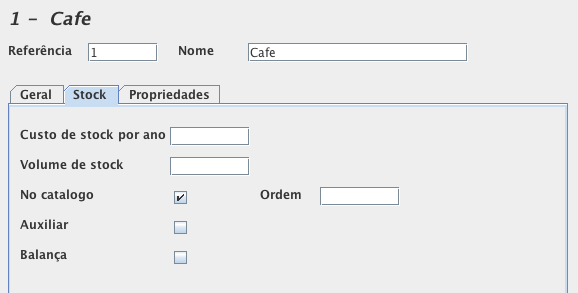
\includegraphics[width=0.4\textwidth]{./imgs_org/produto_stock.png}
  \caption{Separador de defini��o de informa��o de stock de Produtos}
  \label{fig:produto_stock}
\end{figure}

\subsection{Produtos compostos}
� poss�vel definir composi��es de produtos. Produtos normais podem ser compostos
de proutos que se definem como auxiliares. Nesse caso, quando se vende o produto
composto aparece a op��o para acrescentar os seus produtos componentes (n�o �
obrigat�rio). Se acrescentarmos os componentes estes aparecem indentados por
baixo do principal.\newline
\indent Tamb�m se podem vender os produtos auxiliares diretamente.\newline

\subsection{Relat�rios sobre produtos}

\subsubsection{Produtos}
Lista, por categorias, os produtos com os respetivos pre�os de compra (custo),
venda e venda com imposto.

\subsubsection{Etiquetas de produtos}
Lista as fichas dos produtos em formato adequado para afixa��o.

\subsubsection{Cat�logo}
Apresenta o cat�logo de todos os produtos agrupados por fam�liaas/categorias.

\section{Gest�o de Stocks}
Compra de produtos e movimenta��es de stocks.

\subsection{Manuten��o de Stock}
Imprime um recibo relativamente � manuten��o de stock. Permite fazer a
movimenta��o de stock entre armaz�ns. Em caso de movimento imprime um recibo de
sa�da e um recibo de entrada. O valor do produto impresso � o valor de compra
(custo). N�o permite alterar o valor do produto.\newline

\subsection{Di�rio de Stock}
N�o imprime recibo. N�o permite a movimenta��o entre armaz�ms. Serve para
registar as entradas de produtos em armaz�ns da empresa (vindos de
fornecedores). Permite alterar o valor do produto. � �til para, por exemplo,
carregar inicialmente o stock que a empresa tem de todos os produtos.\newline

\subsection{Relat�rios sobre stock}
A aplica��o disponibiliza um conjunto de relat�rio relativos �s movimenta��es de
stock.\newline

\subsubsection{Armaz�ns}
Este relat�rio permite obter o estado do stock actual por armaz�ns e v�rios
filtros relativos a produtos. Apresenta tamb�m os valores monet�rios relativos
aos movimentos de stock.\newline

\subsubsection{Invent�rio corrente}
Relat�rio semelhante ao anterior mas apenas apresenta as unidades dos produtos
em stock.\newline

\subsubsection{Invent�rio corrente ``broken''}
Este relat�rio apresenta os produtos que estejam abaixo do n�vel m�nimo de stock
que foi definido na especifica��o do produto. Note-se que apenas s�o
considerados produtos para os quais tenham sido definidos os limites de
seguran�a de stock.\newline

\subsubsection{Detalhes do invent�rio corrente}
Este relat�rio apresenta as movimenta��es de stock detalhadas por
armaz�m.\newline

\subsubsection{Invent�rio di�rio}
Permite obter os movimentos de stock entre datas, por armaz�m e raz�o do
movimento.\newline

\subsubsection{Detalhes do invent�rio di�rio}
Relat�rio semelhante ao anterior mas com detalhe relativo aos atributos
de produto (caso existam).\newline

\section{Clientes}
A janela de administra��o de clientes permite fazer a gest�o dos dados
associados aos clientes assim como executar relat�rios relativos a clientes. A
Figura ~\ref{fig:clientes} apresenta a janela de administra��o de
clientes.\newline

\begin{figure}[h!]
  \centering
      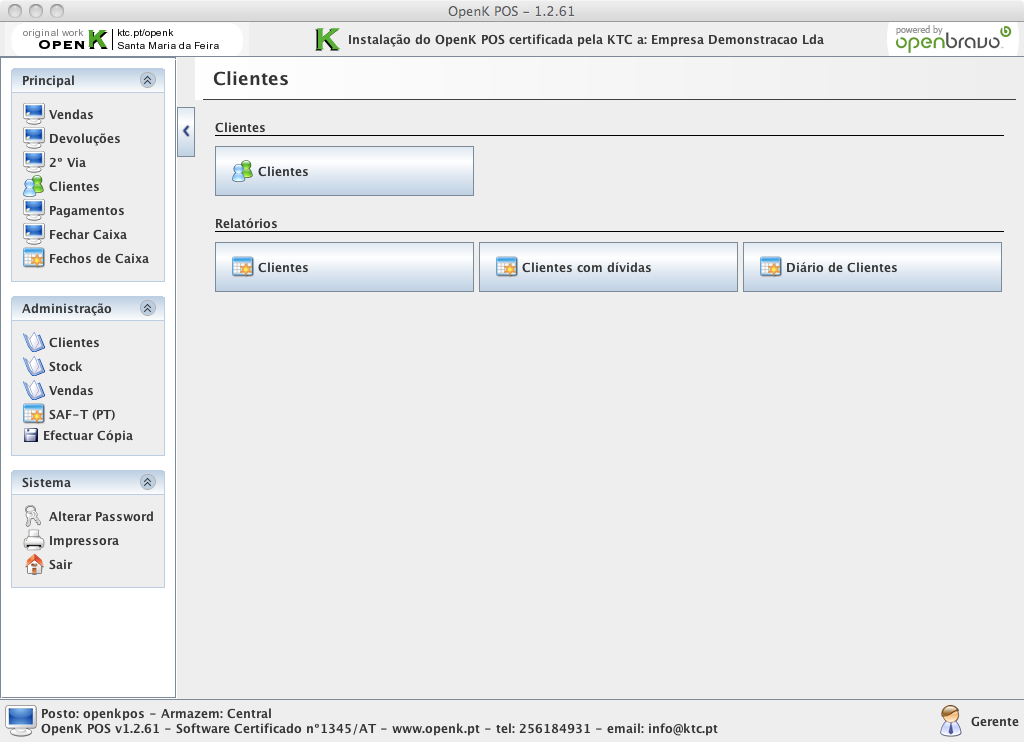
\includegraphics[width=0.8\textwidth]{./imgs_org/clientes.png}
  \caption{Janela de Administra��o de Clientes}
  \label{fig:clientes}
\end{figure}

\begin{itemize}
	\item NIF = N�mero de identifica��o Fiscal. Obrigat�rio
	\item Chave pesquisa = Chave �nica usada para pesquisa do cliente. Obrigat�rio.
	\item Nome = Nome do cliente. Obrigat�rio.
	\item Cart�o = C�digo de barras que pode ser usado num cart�o de cliente para
	identificar o cliente.
	\item Cat de imposto Cliente = Opcional. Permite especificar uma categoria de
	imposto associada ao cliente. Se um cliente tiver uma categoria de imposto
	associado ent�o s� podem ser aplicados a este cliente impostos com a mesma
	categoria de imposto de cliente. Por exemplo, se o cliente � de uma regi�o
	aut�noma cobra-se o IVA da regi�o ou se � um sujeito passivo de uma estado
	membro da UE n�o se cobra IVA.
	\item D�vida m�xima = Permite definir o valor m�ximo da d�vida do cliente.
	\item D�vida do cliente = Apresenta o valor actual da d�vida do cliente.
	\item Data da d�vida = A data do �ltimo valor que ficou em d�vida pelo cliente.
	\item Endere�o
	\begin{itemize}
	  \item Linha de endere�o 1 = Rua do cliente. Obrigat�rio.
	  \item Linha de endere�o 2 = Localidade ou freguesia.
	  \item C�digo postal = C�digo postal. Obrigat�rio.
	  \item Cidade = Obrigat�rio.
	  \item Regi�o = Distrito. Opcional.
	  \item Pa�s = Opcional.
	\end{itemize}
	\item Contacto
	\begin{itemize}
	  \item Dados de contacto do cliente. Opcional.
	\end{itemize}
	\item Notas
	\begin{itemize}
	  \item Informa��o pertinente relativa ao cliente. Esta informa��o pode ser
	  consultada no acto de pagamento de uma venda.
	\end{itemize}
\end{itemize}

\begin{figure}[h!] 
  \centering
      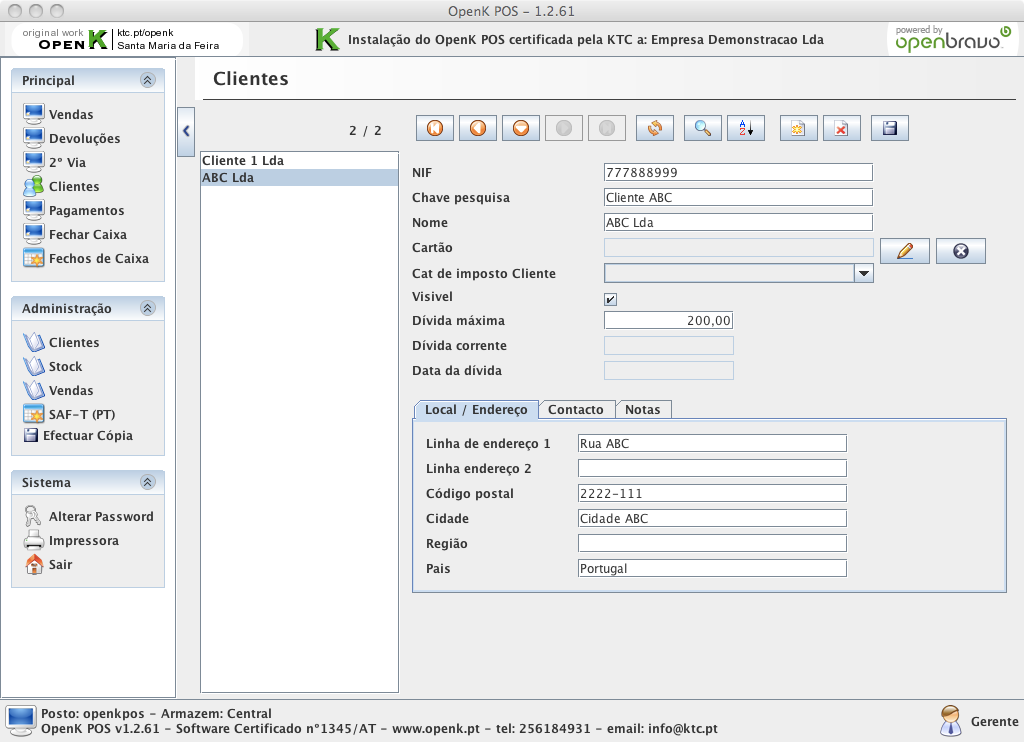
\includegraphics[width=0.8\textwidth]{./imgs_org/editar_cliente.png}
  \caption{Janela de Edi��o de Clientes}
  \label{fig:editar_cliente}
\end{figure}

\subsection{Relat�rios sobre clientes}

\subsubsection{Clientes}
Gera um relat�rio com as fichas dos clientes (ver Figura
~\ref{fig:rel_clientes}).
Se o cliente tiver um cart�o atribu�do ent�o a ficha do cliente inclui o c�digo de barras
relativo ao cart�o do cliente. Para cada cliente aparecem, do lado
esquerdo, a identifica��o do cliente e do lado direito o saldo do
cliente.\newline

\begin{figure}[h!] 
  \centering
      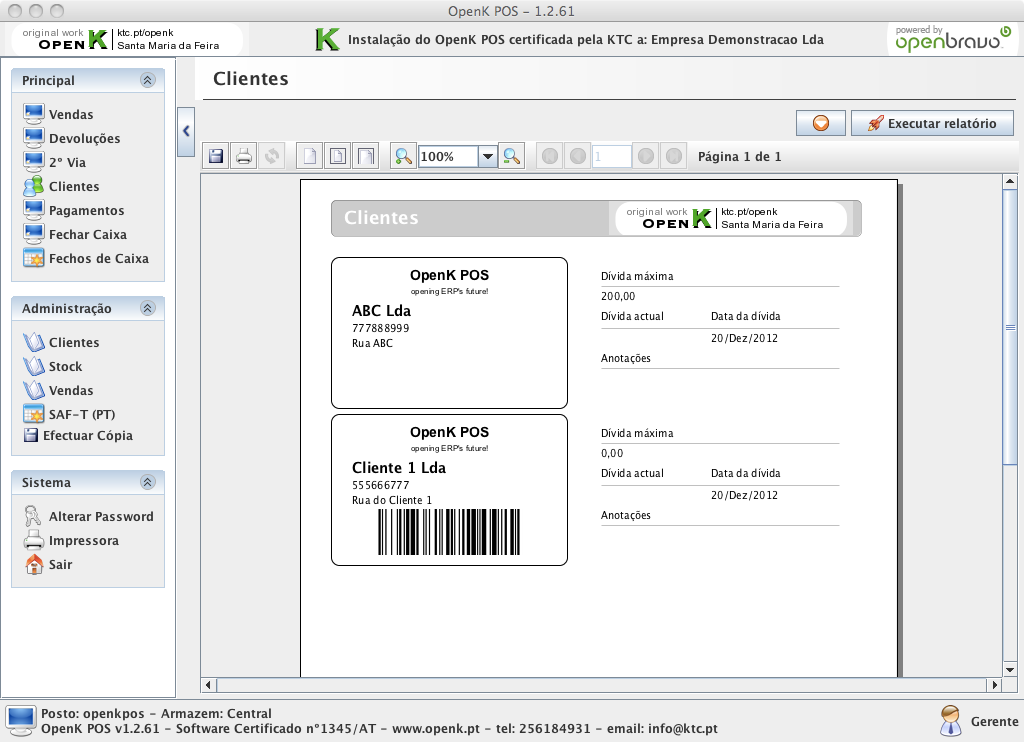
\includegraphics[width=0.8\textwidth]{./imgs_org/rel_clientes.png}
  \caption{Relat�rio de Clientes}
  \label{fig:rel_clientes}
\end{figure}

\subsubsection{Clientes com d�vidas}
Gera um relat�rio com as fichas dos clientes com d�vidas.\newline

\subsubsection{Di�rio de cliente}
Gera um relat�rio com os registos de movimentos de clientes relativos a dividas
e seus pagamentos (ver Figura ~\ref{fig:diario_clientes}).\newline

\begin{figure}[h!] 
  \centering
      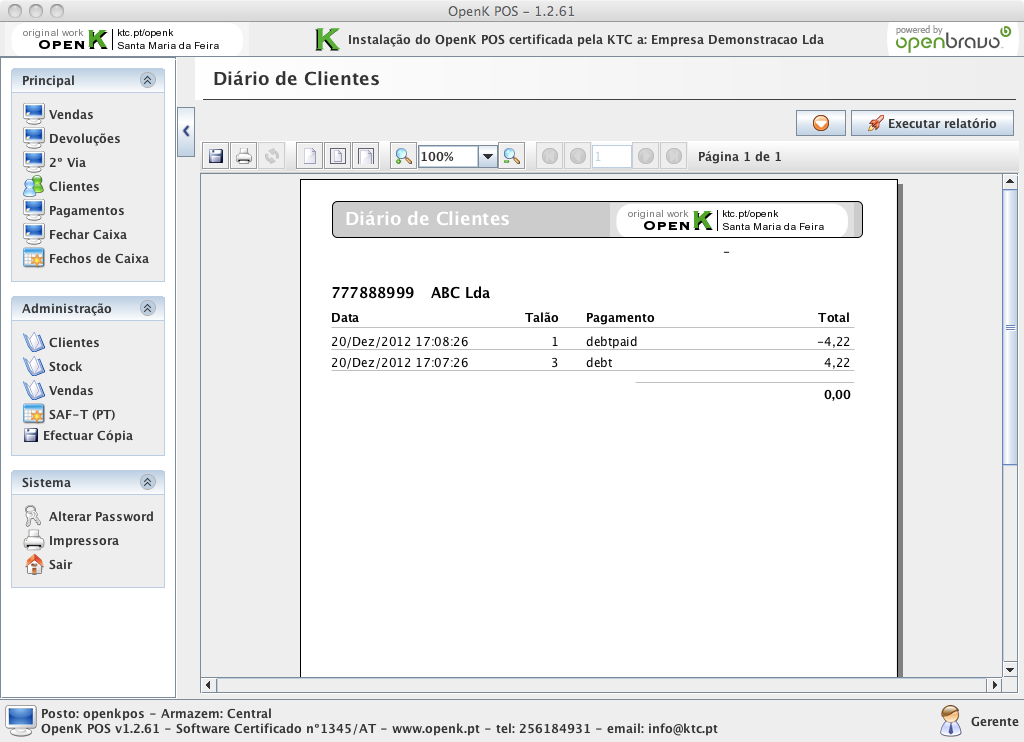
\includegraphics[width=0.8\textwidth]{./imgs_org/diario_clientes.png}
  \caption{Di�rio de movimentos de d�vidas de Clientes}
  \label{fig:diario_clientes}
\end{figure}

\section{Vendas}
Nesta op��o � poss�vel consultar e imprimir dados sobre as
vendas.\newline
Note-se que apenas s�o considerados os dados de caixas fechados.

\subsection{Relat�rio de Caixa por Utilizador}
Imprime os movimentos de caixa por utilizador entre duas datas.\newline

\subsection{Relat�rio de Vendas de Produtos}
Imprime as vendas por produto entre duas datas.\newline

\subsection{Relat�rio de Impostos}
Imprime os impostos das vendas entre duas datas.\newline

\subsection{Relat�rio de Vendas e Impostos}
Imprime os impostos das vendas entre duas datas. Este relat�rio �
adequado para suportar a declara��o peri�dica de IVA.\newline

\subsection{Gr�fico de Vendas}
Apresenta um gr�fico de vendas por utilizador e por datas.

\subsection{Gr�fico de Vendas de Produtos}
Apresenta um gr�fico de vendas por produto e por datas.

\section{Emiss�o do Ficheiro SAF-T PT}
Esta op��o permite gerar o ficheiro SAF-T de acordo com a regulamenta��o da
Autoridade Tribut�ria Portuguesa (Finan�as). Para emitir o ficheiro � necess�rio
especificar um intervalo de datas relativo ao per�odo para o qual desejamos os
dados do SAF-T.

\section{C�pias de Seguran�a}
Esta op��o permite gerar c�pias de seguran�a dos dados da aplica��o. Deve ser
executada com regularidade (uma sugest�o � efectua-la com a periodicidade do
fecho de caixa).\newline

\begin{bclogo}[couleur=blue!30, arrondi=0.1, logo=\bclampe, ombre=true]{�
poss�vel automatizar a gera��o de c�pias de seguran�a} Para tal deve solicitar
o servi�o aos t�cnicos da KTC. Ap�s a falha do sistema a reposi��o de c�pias de
seguran�a deve ser solicitada aos t�cnicos da KTC.
\end{bclogo}




 

\chapter{Opera��es}
\label{ch:operacoes}

\section{Vendas}
Insere-se o c�digo do produto que pode ser um c�digo de barras de 13
d�gitos ou um c�digo introduzido manualmente (mas que � o mesmo que o
que foi introduzido na ficha do produto mas tem menos de 13 d�gitos). Se
introduzirmos um c�digo de barras de cliente a aplica��o assume o
cliente da venda de forma autom�tica (� um c�digo de barras que inicia
pela letra 'c').\newline

\section{Devolu��es}
Esta op��o permite registar devolu��es de documentos de venda. � �til quando o
cliente devolve produtos de uma venda ou quando, por alguma raz�o, existem erros
no documento de venda que devem ser corrigidos. � gerado um documento de
``anula��o'' da venda que fica registado com um documento de devolu��o. Este
documento de devolu��o faz refer�ncia ao documento de venda original que est� a
anular (total ou parcialmente).\newline
Se o objectivo da devolu��o � a corre��o de um documento de venda com erros o
que se deve fazer � a devolu��o da totalidade do documento de venda original e
seguidamente usar a op��o de vendas para registar a venda de forma
correta.\newline

\section{Segunda via}
Esta op��o permite imprimir segundas vias dos coumentos de venda.\newline

\section{Clientes}
Permite consultar o estado da conta corrente dos clientes e saldar as
dividas de clientes (emite um recibo do valor que o cliente pagou e
daquilo que ainda ficou em divida).\newline
Pode-se pesquisar o cliente pelo seu cart�o (pode ser lido por c�digo de
barras).\newline

\section{Pagamentos}
Permite registar no caixa a entrada de dinheiro sem ser por recebimento de
venda.\newline

\section{Fecho de Caixa}
Permite consultar o estado actual do caixa, imprimir o estado do caixa
ou fechar o caixa. Sempre que o caixa � fechado � impresso um pequeno
relat�rio sobre o fecho.\newline
Sempre que se fecha o caixa o sistema automaticamente abre um novo
caixa.\newline
Pode-se fechar o caixa com a periodicidade desejada (todos os dias, uma vez por
semana, quando necess�rio).\newline

\section{Relat�rio de fecho de caixa}
Permite obter um relat�rio de fechos de caixa entre datas.\newline









\chapter{Licen�a}
\label{ch:licenca}

O software OpenK POS (http://www.openk.pt) � distribu�do segundo a licen�a GPL
v3 tal como publicado pela Free Software Foundation (consultar a sec��o 6.3 ou
http://www.gnu.org/licenses/). Esta licen�a aplica-se ao c�digo da autoria da
KTC Knowledge Teaching Center Lda assim como ao c�digo do projecto base
Openbravo POS (http://www.openbravo.com). Algumas bibliotecas do software
Openbravo t�m uma licen�a diferente. Estas est�o desctiminadas no Openbravo
POS.\newline
Em conformidade com a licen�a GPL v3 o c�digo fonte do OpenK POS est� acess�vel
de forma id�ntica ao do respectivo c�digo bin�rio (i.e., aplica��o
execut�vel).\newline
A disponibiliza��o do c�digo fonte da aplica��o que est� relacionado com ao
certifica��o junto da Autoridade Tribut�ria (Finan�as) � efectuada medianta
compromisso comprovado de que a entidade/pessoa que tem acesso a esse c�digo ir�
certificar a sua utiliza��o no software derivado junto da Autoridade Tribut�ria
(Finan�as). Em adi��o, o receptor desse c�digo fonte deve declarar por escrito
que incluir� obriga��o semelhante no seu software derivado e que n�o usar� o
conhecimento adquirido com o c�digo fonte de forma que permita violar a
certifica��o do software original OpenK e dos seus softwares derivados.\newline
Para al�m deste requisito, o software derivado do OpenK POS deve obedecer ainda
ao descrito na sec��o 6.2.

\section{Certifica��o AT/Finan�as}
O software OpenK POS encontra-se devidamente certificado pela Autoridade
Tribut�ria Portuguesa (Finan�as). O acordo de certifica��o entre a KTC e a AT
implica que certos recursos privados derivados da certifica��o n�o podem ser
distribu�dos.\newline

\begin{bclogo}[couleur=blue!30, arrondi=0.1, logo=\bclampe,
ombre=true]{Condi��o de certifica��o da aplica��o} Note-se que apenas as
instala��es do OpenK POS efectuadas e mantidas pela KTC est�o certificadas pela AT. Assim, ap�s o termino do contrato de servi�os entre a KTC e o Cliente a
aplica��o deixa de se considerar certificada e deve ser removida
permanentemente.
\end{bclogo}

\section{Extens�es e Produtos Derivados}
Qualquer software baseado no OpenK POS deve obedecer � mesma licen�a GPL v3 e
para al�m disso conter em todos os ecr�s o logotipo do OpenK indicando que se
trata de uma extens�o e/ou deriva��o do software OpenK POS. Deve ainda ser claro
que a KTC n�o tem qualquer responsabilidade sobre a extens�o e/ou
deriva��o.\newline

\begin{bclogo}[couleur=blue!30, arrondi=0.1, logo=\bclampe,
ombre=true]{Apenas as instala��es do OpenK POS efectuadas e mantidas pela KTC
est�o certificadas pela AT} Assim, ap�s o termino do contrato de servi�os entre
a KTC e o Cliente a aplica��o deixa de se considerar certificada.
\end{bclogo}\newline

\noindent Todos os ecr�s/janelas de software que estenda ou seja um
derivado do OpenK POS devem conter no canto superior esquerdo do topo do ecr�
(ver Figura ~\ref{fig:topo_ecra}) o logotipo das deriva��es ou extens�es ao
OpenK POS (ver Figura ~\ref{fig:derivedwork}) em lugar do logotipo que marca
a vers�o original do OpenK (ver Figura ~\ref{fig:originalwork}). � ainda
obrigat�ria a inclus�o do logotipo do Openbravo no canto superior direito de todos os ecr�s/janelas, tal como tamb�m se pode observar na Figura 15. \textbf{A mensagem central e o t�tulo da janela devem ser adaptados de forma a identificar claramente que se
trata de uma extens�o ou deriva��o do OpenK e n�o da vers�o original.}\newline

\begin{figure}[h!] 
  \centering
      
\includegraphics[width=0.8\textwidth]{./imgs_org/topo_ecra.png}
  \caption{Linha de topo do ecr�}
  \label{fig:topo_ecra}
\end{figure}

\begin{figure}[h!] 
  \centering
      
\includegraphics[width=0.3\textwidth]{./imgs_org/derivedwork.png}
  \caption{Logotipo OpenK para software derivado e extens�es}
  \label{fig:derivedwork}
\end{figure}

\begin{figure}[h!] 
  \centering
      
\includegraphics[width=0.3\textwidth]{./imgs_org/originalwork.png}
  \caption{Logotipo original do OpenK}
  \label{fig:originalwork}
\end{figure}

\section{Texto integral da licen�a GPL}

\verbatiminput{./gpl.txt}




\bibliographystyle{plain}
\bibliography{manual}

\end{document}